
\section{Evaluation and experience}
\label{sec:eval-exper}

The Coq proof assistant serves as a tool for implementing FCSL's
metatheory and as a language for writing and verifying concurrent
programs.
%
The formalization of the metatheory, which includes the semantic
model, structural lemmas and a number of useful libraries of lemmas,
specific for the whole development or particular examples (\eg,
getters, theory of PCMs, heaps, arrays, \etc.), is about 17.2 KLOC
size.

\subsection{Statistics for the case studies}
\label{sec:stat-proof-sizes}

{
%\setlength{\belowcaptionskip}{-10pt} 
\begin{table}[t]
{%\footnotesize
%\sffamily\small % tabular data either 10pt times, or 9pt helvetica
\centering
\begin{tabular}{|@{\ }l@{\ \ \ }||@{\ }c@{\ }|@{\ }c@{\ }|@{\ }c@{\ }|@{\ }c@{\ }|@{\ }c@{\ }|@{\ }c@{\ }||@{\ }r@{\ }|}
  \hline
  \textbf{Program} &  
  {Libs} & {Conc} & {Acts} &
  {Stab} & {Main} & \textbf{Total}
  & \textbf{Build~~~}   
  \\ \hline \hline 
  CAS-lock & 63 & 291 & 509 & 358 & 27 & 1248 & 1m~~~1s
  \\
  Ticketed lock & 58 & 310 & 706 & 457 & 116 & 1647 & 2m~46s
  \\
  CG increment & 26 & - & - & - & 44 & 70 & 8s
  \\
  CG allocator & 82 & - & - & - & 192 & 274 & 14s
  \\
  Pair snapshot & 167 & 233 & 107 & 80 & 51 & 638 & 4m~~~7s 
  \\
  Treiber stack & 56 & 323 & 313 & 133  & 155 & 980 & 2m~41s
  \\
  Spanning tree & 348 & 215 & 162 & 217 & 305 & 1247 & 1m~11s
  \\
  Flat combiner & 92 & 442 & 672 & 538 & 281 & 2025 &  10m~55s
  \\ 
  Sequential stack & 65 & - & - & - & 125 & 190 & 1m~21s
  \\
  FC-stack & 50 & - & - & - & 114 & 164 & 44s
  \\
  Producer/Consumer & 365 & - & - & - & 243 & 608 & 2m~43s
  \\[2pt] \hline
\end{tabular}
\vspace{15pt}
\caption{ 
  Statistics for implemented programs: lines of code for program-specific libraries \intab{Libs},
  definitions of concurroids and decorations \intab{Conc}, actions \intab{Acts},
  stability lemmas \intab{Stab}, spec and proof sizes of the main
  functions \intab{Main}, total LOC count \intab{\textbf{Total}}, and build
  times \intab{\textbf{Build}}.
} 
\label{tab:locs}
}
\end{table}}
%
We evaluated FCSL by implementing, specifying and verifying a number
of characteristic concurrent programs and structures. The simplest
fine-grained structure is a lock, and we implemented two different
locking protocols: CAS-based spinlock and a ticketed
lock~\cite{DinsdaleYoung-al:ECOOP10}. Both locks instantiate a uniform
abstract lock interface, and are used by coarse-grained programs,
performing concurrent incrementation of a pointer and memory
allocation. In addition to the spanning tree algorithm and the flat
combining construction, we also implemented such fine-grained programs
as an atomic pair snapshot~\cite{Qadeer-al:TR09,Liang-Feng:PLDI13} and
non-blocking stack~\cite{Treiber:TR}, both given specs via a PCM of
time-stamped action histories in the spirit of
linearizability~\cite{Sergey-al:ESOP15,Herlihy-Wing:TOPLAS90}, as well
as several client programs: a sequential stack (obtained from Treiber
stack via hiding), FC-based stack, and a Treiber stack-based
concurrent Producer/Consumer.
%
The PCMs employed by formalizations of the case studies are:
%
\begin{itemize}[itemindent=0pt] 

\item disjoint sets~\cite{Nanevski-al:ESOP14} (spanning tree, FC, ticketed lock);
\item heaps~\cite{LeyWild-Nanevski:POPL13,Calcagno-al:LICS07} (thread-local state);
\item natural numbers with addition and zero~\cite{LeyWild-Nanevski:POPL13} (CG increment);
\item mutual exclusion PCM~\cite{LeyWild-Nanevski:POPL13,Nanevski-al:ESOP14} (CAS-lock, ticketed lock, FC);
\item time-stamped histories~\cite{Sergey-al:ESOP15} (pair snapshot, Treiber stack, producer/consumer);
\item client-provided PCMs~\cite{LeyWild-Nanevski:POPL13,Nanevski-al:ESOP14} (FC, locks);
\item \emph{lifted} PCMs---products of basic PCMs~\cite{LeyWild-Nanevski:POPL13,Nanevski-al:ESOP14} (FC, locks). 

\end{itemize}
%
All these cases are treated uniformly by in the proofs conducted in FCSL
framework, due to the unifying algebraic structure.


Table~\ref{tab:locs} presents some statistics \wrt implemented
programs in terms of LOCs and build times.  The program suite was
compiled on a 2.7 GHz Intel Core i7 OS X machine with 8~Gb RAM, using
Coq~8.4pl4 and Ssreflect~1.4.
%
We didn't rely on any advanced proof automation in the proof scripts,
which would, probably, decrease line counts at the expense of
increased compilation times. Notably, for those programs that required
implementing new primitive concurroids (\eg, locks or Treiber stack),
a large fraction of an implementation is due to proofs of properties
of transitions and actions, as well as stability-related lemmas, while
the sizes of proofs of the main programs' specs are always relatively
small.
% %
% \ab{Are the proof sizes given by the Main column? Also, any thoughts
%   on why Flat combiner build time is longer than others?}
% %
% \is{Yes, these are the proofs (the caption explains this now). As for
%   the FC, we don't quite know. Must be something of the Coq
%   unification itself.}

\subsection{Composition of the specifications and proofs}
\label{sec:comp-spec-proofs}

%
{
\setlength{\belowcaptionskip}{-15pt}  
\begin{figure}[t]
\centering
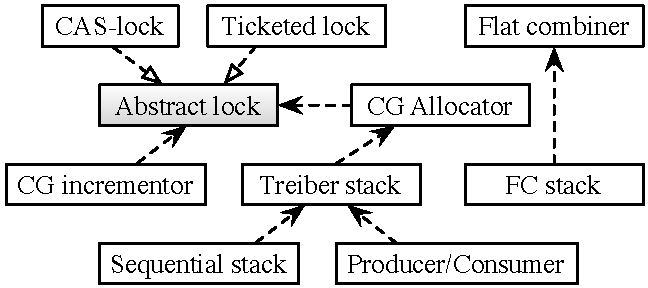
\includegraphics[width=0.8\textwidth]{dependencies.pdf}
%\vspace{-5pt}       
\caption{Dependencies between concurrent libraries.}
\label{fig:deps}
\end{figure}
}
%
Our development is inherently compositional, as illustrated by the
dependency diagram on Figure~\ref{fig:deps}. For example, both lock
implementations are instances of the abstract lock interface,
%
% in the spirit of concurrent abstract
% predicates~\cite{DinsdaleYoung-al:ECOOP10}, 
%
which is used to implement and verify the allocator, which is then
employed by a Treiber stack, used as a basis for sequential stack
and producer/consumer implementations. In principle, we could
implement an abstract interface for stacks, too, to unify the Treiber
stack and the FC-stack, although, we didn't carry out this exercise.

\subsection{Concurroids reuse}
\label{sec:concurroids-reuse}

As hinted by Table~\ref{tab:locs}, not every concurrent program
requires implementing a new primitive concurroid: typically this is
done only for libraries, so library clients can reason out of the
specifications.  Table~\ref{tab:concur} shows that the reuse of
concurroids is quite high, and most of the programs make consistent
use of the concurroid for thread-local state and locks (abstracted
through the corresponding interface), as well as of those required by
the used libraries (\eg, Treiber or FC).
%
{
\setlength{\belowcaptionskip}{-10pt} 
\begin{table}[t]
{
%\footnotesize
%\sffamily\small % tabular data either 10pt times, or 9pt helvetica
\centering
\begin{tabular}{@{\ \ }l@{\ \ \ }c@{\ \ \ }c@{\ \ }c@{\ }c@{\!\!\!}c@{\!}c@{\!\!\!\!}c}
  \textbf{Program} &  
  \rot{\cccode{Priv}} & \rot{\cccode{CLock}} & \rot{\cccode{TLock}} &
  \rot{\cccode{ReadPair}} & \rot{\cccode{Treiber}} & \rot{\cccode{SpanTree}}
  & \rot{\cccode{FlatCombine}}   
  \\ \hline 
  CAS-lock & \yep & \yep &&&&&
  \\
  Ticketed lock & \yep && \yep &&&
  \\
  CG increment & \yep & \yepl & \yepl & & & &
  \\
  CG allocator & \yep & \yepl & \yepl &&&&
  \\
  Pair snapshot & & & & \yep &&&
  \\
  Treiber stack & \yep & \yepa & \yepa & & \yep &&
  \\
  Spanning tree & \yep & & & & & \yep &
  \\
  Flat combiner & \yep & \yepa & \yepa & & & & \yep
  \\ 
  Sequential stack & \yep & \yepa & \yepa & & \yep & &
  \\
  FC-stack & \yep & \yepa & \yepa & & & & \yep
  \\
  Producer/Consumer & \yep & \yepa & \yepa & & \yep & &
  \\[2pt] \hline
  \\
\end{tabular}
%\vspace{-5pt}
\caption{
  % 
  Primitive concurroids (in column headings) employed by different programs. Two lock
  concurroids, for CAS-based and ticketed locks, are interchangeable, as they implement the same abstract interface
  (indicated by \yepl).  
%
}
\label{tab:concur}
}
\end{table}
}
%

